\chapter{Hierarchical Physics Development}
\label{chapter: Hierarchical_Physics_Development}

Chapter 7 of the CCPP v6 Technical Documentation (\url{https://ccpp-techdoc.readthedocs.io/en/v6.0.0/}) provides an overview of the tools supported by the Single Column Model (SCM) to faciliate hierarchical system development (HSD)

\section{Background}

Developing and implementing a new physics parameterization for use in an operational setting requires extensive testing and evaluation. This is to ensure that new developments aren’t yielding unexpected results and that all computational considerations are being met. From a scientific perspective, this process should be incremental and hierarchical, i.e. using HSD which follows a systems-engineering approach, i.e. initial testing of simple idealized cases that focus on small elements (e.g., physics schemes) of an Earth System Model (ESM) first in isolation, then progressively connecting elements with increased coupling between ESM components at the different HSD steps. HSD includes SCMs (including individual elements within the SCM), Small-Domain, Limited-Area and Regional Models, all the way up to complex fully-coupled ESMs with components for atmosphere/chemistry/aerosols, ocean/waves/sea-ice, land-hydrology/snow/land-ice, and biogeochemical cycles/ecosystems, a subset of which (i.e. atmosphere+land and specified ocean conditions) has traditionally addressed Numerical Weather Prediction (NWP) needs. HSD is end-to-end in that it includes data ingest and quality control, data assimilation, modeling, post-processing, and verification. The requirements for advancing from one HSD step to the next are appropriate metrics/benchmarks for ESM (or ESM components or elements) performance, many of which are at the physical process level, plus the necessary forcing data sets to drive and validate models. Datasets for use in different HSD steps are obtained from measurements (e.g. field programs and observational networks), ESM output, or idealized conditions (often used to “stress-test” schemes/elements/system components, among many other options). It is important to note that the HSD process is concurrent and iterative, i.e. more complex HSD steps can provide information to be used at simpler HSD steps, and vice versa. This also includes understanding spatial and temporal dependencies in model physics, and the need for consistency in those solutions in models between higher-resolution/regional short-range, global medium/extended-range, and subseasonal-to-seasonal time scales.

The CCPP-SCM provides developers working within CCPP-compliant host models the ability to test their physics innovations without having to worry about the coupling to the dynamical core. This is a critical step in the model development hierarchy, providing insight on how an introduced physics change can modify the evolution of the internal physics state. However, there are still challenges, most notably the interactions between introduced changes and the other physics schemes in the suite.

\section{CCPP Suite Simulator}

\subsection{Overview}

The CCPP Suite Simulator is a CCPP compliant physics scheme that provides the ability to turn on/off physical processes in a Suite Definition File (SDF), using namelist options. This simulator `piggybacks' on an existing SDF, replacing physics tendencies with data-driven tendencies (\ref{fig:CSS_tendency_schematic}). 

\begin{figure}[h]
    \centering
    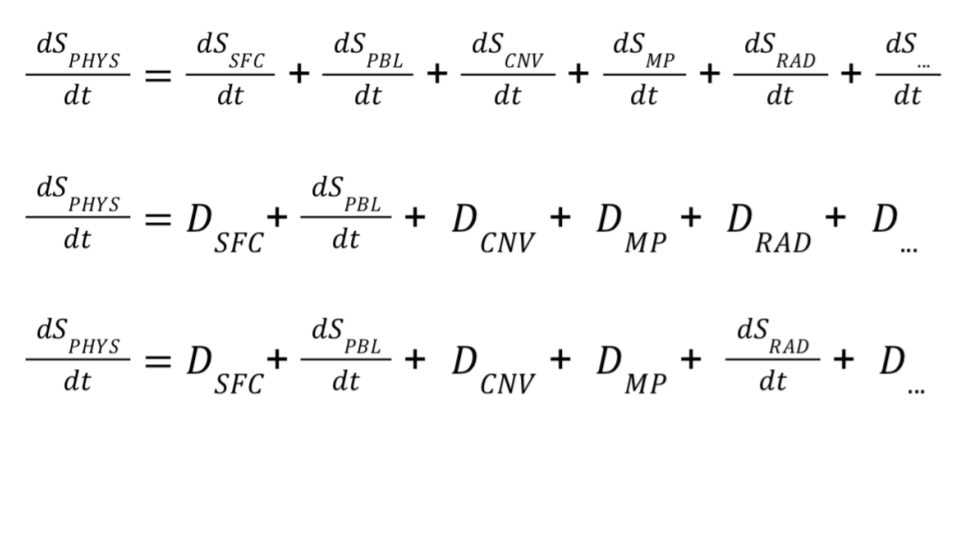
\includegraphics[width=0.80\textwidth]{images/CSS_tendency_schematic.png}
    \caption{Equation for internal physics state evolution for process-split physics suite, where S is the prognostic state and D are simulated data tendencies. Top) Standard Suite Definition File; Middle) Active PBL physics with simulated tendencies for other schemes; Bottom) Active PBL and radiation, with simulated tendencies for other schemes.}
    \label{fig:CSS_tendency_schematic}
\end{figure}

\subsection{Process-split vs. Time-split Physics Process}

Process-split physics processes are schemes that share a common input state, whereas time-split processes use the state provided by the previous physics process. A SDF can be any combination of time-split and process-split schemes, just as long as the appropriate interstitial schemes are created to couple the physics schemes.

\subsection{About the CCPP Suite Simulator}

The CCPP Suite Simulator (CSS) emulates the evolution of the internal physics state provided by the SDF. There are different deployments of the suite simulator, depending on the role(s) and order of the physical processes in the SDF we are emulating (e.g. time vs. process-split), that need further attention. For instance, SDFs consisting of only process-split physics schemes can be handled simply by adding the simulator to the end of the SDF, since for process-split schemes the order is not critical to the evolution of the internal physics state. On the other hand, for SDFs that contain time-split processes, where the simulator is added is important to preserve the order of the internal state evolution.

\subsection{Python Dependencies}
\label{subsection: pydepend}
The scripts here require a few python packages that may not be found by default in all python installations. There is a YAML file with the python environment needed to run the script in \execout{ccpp-scm/environment\_suite\_sim.yml}. To create and activate this environment using conda:

Create environment (only once):

\execout{> conda env create -f environment-suite-sim.yml}

This will create the conda environment \execout{scm\_suite\_sim}


Activate environment:

\execout{> conda activate scm\_suite\_sim}

\subsection{Enabling the CCPP Suite Simulator}

To use the CSS in the CCPP-SCM three modifications need to be made:

\begin{enumerate}
\item Add CSS, and any interstitial schemes needed for coupling the CSS to the host (e.g. SCM), to an existing CCPP SDF (or create a new SDF).
\item Set \execout{do\_ccpp\_suite\_sim = .true.} in the GFS physics namelist, \execout{gfs\_physics\_nml}
\item Modify, or create new, namelist that has the options needed to activate the CSS.
\end{enumerate}

\subsection{Modifying the CCPP Suite Definition File}

The SDF needs to be modified to include the CSS scheme, and any interstitial schemes needed for your host application. Here we will illustrate how to use the CSS within SCM (UFS) physics, for which all applications use a physics SDF with mixture of process-split and time-split physics schemes.
In general,
\begin{itemize}
\item for SDFs that contain ONLY process-split schemes, the CSS can be added to the end of the SDF for all configurations. In this case we have the flexibility to switch ``on/off'' any combination of active physics and simulated physics at runtime, via namelist, with the same modified SDF.
\item when using SDFs that contain ONLY time-split schemes, the CSS needs to be added before and after each scheme you want to switch ``on/off''. So one could add calls to the CSS between each process in the SDF to obtain total flexibility, or just around the schemes they are interested in.
\end{itemize}

In the examples below we will demonstrate how to modify SDFs to use the CSS for SCM (UFS) physics applications, \ref{section:Suite_with_Active_Radiation} and \ref{section:Suite_with_Active_cldmp}.

\subsection{Namelist for the CCPP Suite Simulator}

The CSS has its own namelist, \execout{ccpp\_suite\_sim\_nml}, that needs to be added to the physics namelists used by the SCM.

\lstinputlisting[
                 basicstyle=\scriptsize\ttfamily,
                 label=lst_css_nml_ex1,
                 caption=Example namelist for CCPP Suite Simulator.
                 ]{./css_nml.txt}

\begin{itemize}
\item \execout{suite\_sim\_file}: Input file with simulated data tendencies (See \ref{section:Creating_Custom_Data_for_Simulator} for how to create input file from SCM output).
\item \execout{nprc\_sim}: Number of physical processes in the input data.
\item \execout{prc\_XYZ\_cfg}: Configuration for physical process XYZ.
\begin{itemize}
\item 0 - Active scheme; 1 - Use data
\item 0 - Process-split scheme; 1 - Time-split scheme
\item Index for scheme order (1 - \execout{nprc\_sim})
\end{itemize}
\end{itemize}

For example, in Listing \ref{lst_css_nml_ex1}, there are two active schemes, longwave and shortwave radiaiton, and five simulated schemes: PBL, gravity-wave drag, deep/shallow convection, and cloud microphysics. The radiation, gravity-wave drag and PBL schemes are all process-split, whereas convection and cloud microphysics are time-split. 

\subsection{Creating Custom Data for Simulator}
\label{section:Creating_Custom_Data_for_Simulator}

Navigate to \execout{ccpp-scm/scm/etc/scripts/ccpp\_suite\_sim}

Provided with the SCM are scripts to generate data for the suite simulator using output from a previous SCM run. The first script, \execout{create\_1D\_CSSdata.py}, extracts the physics tendencies from a user specified time interval, which are used for constant forcing in the suite simulator. The other script, \execout{create\_2D\_CSSdata.py}, creates a two-dimensional forcing dataset. The suite simulator interpoaltes these forcings in time.

\begin{enumerate}
\item Run the SCM twice using the TWPICE case with the \execout{GFS\_v16} and \execout{GFS\_v17\_p8} suites.
\begin{lstlisting}[language=bash]
cd ccpp-scm/scm/bin
./run_scm.py -c twpice -s SCM_GFS_v16
./run_scm.py -c twpice -s SCM_GFS_v17_p8
\end{lstlisting}
\item Create 2D forcing data for the CSS, using SCM output from TWPICE case with \execout{GFS\_v16} suite.
\begin{lstlisting}[language=bash]
cd ccpp-scm/scm/etc/scripts/ccpp_suite_sim
./create_2D_CSSdata.py --cases twpice --suites SCM_GFS_v16
\end{lstlisting}
\item Create constant forcing data for the CSS, using SCM output, at forecast time 3600s, from TWPICE case with \execout{GFS\_v17\_p8} suite.
\begin{lstlisting}[language=bash]
cd ccpp-scm/scm/etc/scripts/ccpp_suite_sim
./create_1D_CSSdata.py --cases twpice --suites SCM_GFS_v17_p8 --time 3600
\end{lstlisting}
\end{enumerate}

The data file will be written to \execout{ccpp-scm/scm/etc/scripts/ccpp\_suite\_sim/} with the following format, \execout{data\_CSS\_DIM.CASES.SUITES.nc}.

\subsection{Example 1: Suite with Active Radiation}
\label{section:Suite_with_Active_Radiation}

For this example we will use the two-dimensional forcing data from \ref{section:Creating_Custom_Data_for_Simulator}. 

First, we need to modify the SDF to include the CSS, \execout{ccpp\_suite\_simulator.F90} and an additional interstital scheme to couple to the GFS physics, \execout{GFS\_ccpp\_suite\_sim\_pre.F90} (See \ref{fig:CSS_SDF_ex1}).

\begin{figure}[t]
    \centering
    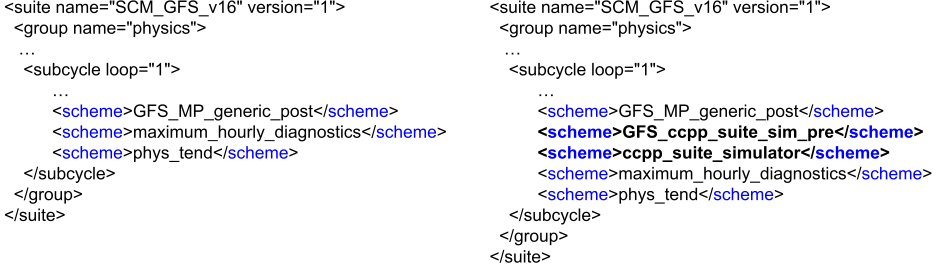
\includegraphics[width=0.80\textwidth]{images/SDF_changes_for_CSS_ex1.png}
    \caption{Changes to GFS v16 physics SDF to include CCPP suite simulator for \execout{active} radiation parameterization. All other parameterizations are replaced by simulated data.}
    \label{fig:CSS_SDF_ex1}
\end{figure}

Next, the physics namelist needs to be configured to:
\begin{enumerate}
\item Add data file, \execout{suite\_sim\_file} created in \ref{section:Creating_Custom_Data_for_Simulator} to the namelist.
\item Turn ``off'' all schemes except the radiation (see Listing \ref{lst_css_nml_ex1})
\end{enumerate}

Finally, we rebuild the SCM with the modified SDFs to include the CSS, and run the SCM  using TWPICE case with the modified \execout{GFS\_v16} suite.
\begin{lstlisting}[language=bash]
cd ccpp-scm/scm/bin
cmake ../src -DCCPP_SUITES=SCM_GFS_v16
./run_scm.py -c twpice -s SCM_GFS_v16
\end{lstlisting}

\subsection{Example 2: Suite with Active Cloud Microphysics}
\label{section:Suite_with_Active_cldmp}

For this example we will use the constant forcing data from \ref{section:Creating_Custom_Data_for_Simulator}.

First, we need to modify the SDF to include the CSS, \execout{ccpp\_suite\_simulator.F90} and an additional interstital scheme to couple to the GFS physics, \execout{GFS\_ccpp\_suite\_sim\_pre.F90} (See \ref{fig:CSS_SDF_ex2}).

\begin{figure}[h]
    \centering
    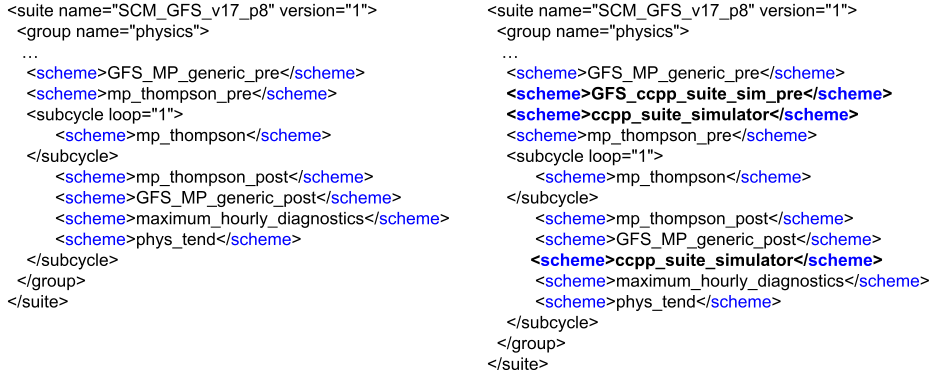
\includegraphics[width=0.80\textwidth]{images/SDF_changes_for_CSS_ex2.png}
    \caption{Changes to GFS v17 Prototype 8 physics SDF to include CCPP suite simulator for \execout{active} cloud microphysics parameterization. All other parameterizations are replaced by simulated data.}
    \label{fig:CSS_SDF_ex2}
\end{figure}

Next, the physics namelist needs to be configured to:
\begin{enumerate}
\item Add data file, \execout{suite\_sim\_file} created in \ref{section:Creating_Custom_Data_for_Simulator} to the namelist.
\item Turn ``off'' all schemes except the cloud microphysics (see Listing \ref{lst_css_nml_ex2})
\end{enumerate}

\lstinputlisting[
                 basicstyle=\scriptsize\ttfamily,
                 label=lst_css_nml_ex2,
                 caption=Example namelist for CCPP Suite Simulator with active cloud microphysics.
                 ]{./css_nml_ex2.txt}

Finally, we rebuild the SCM with the modified SDFs to include the CSS, and run the SCM  using TWPICE case with the modified \execout{GFS\_v17\_p8} suite.
\begin{lstlisting}[language=bash]
cd ccpp-scm/scm/bin
cmake ../src -DCCPP_SUITES=SCM_GFS_v17_p8
./run_scm.py -c twpice -s SCM_GFS_v17_p8
\end{lstlisting}

\subsection{Plotting tools}
\label{section:plotting_tools}

Additionally, plotting scripts provided in \execout{ccpp-scm/scm/etc/scripts/ccpp\_scheme\_sim}:

\begin{enumerate}
\item
\begin{lstlisting}[language=bash]
./plt_scmout_2d.py [-h] -n CASE_NAME -sdf SDF -nmls NMLS -vars VAR1 VAR2 VAR3
\end{lstlisting}

Mandatory arguments:
\begin{enumerate}
\item \exec{-{}-case\_name (-n)} name of case
\item \exec{-{}-suite (-sdf)} CCPP suite definition file
\item \exec{-{}-nml\_list (-nmls)} namelists, separated by a space
\item \exec{-{}-var\_list (-vars)} varaibles to plot, separated by a space
\end{enumerate}

\item
\begin{lstlisting}[language=bash]
./plt_scmout_3d.py [-h] -n CASE_NAME -sdf SDF -nmls NMLS -vars VAR1 VAR2 VAR3 -time TIME
\end{lstlisting}

Mandatory arguments:
\begin{enumerate}
\item \exec{-{}-case\_name (-n)} name of case
\item \exec{-{}-suite (-sdf)} CCPP suite definition file
\item \exec{-{}-nml\_list (-nmls)} namelists, separated by a space
\item \exec{-{}-var\_list (-vars)} varaibles to plot, separated by a space
\item \exec{-{}-time\_plot (-time)} time to plot, in seconds
\end{enumerate}

\end{enumerate}
